\section*{Question 1}

Determine the interior, closure and border of the following sets:

\begin{enumerate}[label=(\alph*)]
\item $S_1 = \{x \in \mathbb{R}^2 | x_1^2 + x_2^2 \leqslant 1, x_2 > 1 \}$

\item $S_2 = \{x \in \mathbb{R}^2 | x_1^2 + x_2^2 \leqslant 1, x_1 + x_2 = 1.4 \}$

\item $S_3 = \{x \in \mathbb{R}^2 | x_1^2 + x_2^2 \leqslant 1, x_1 + x_2 = 1.5 \} $
\end{enumerate}

\subsection*{Solution}

\begin{enumerate}[label=(\alph*)]
\item Set $S_1$ can be represented as the intersection of two sets $S_{\text{sub}_1} = \{x \in \mathbb{R}^2 | x_1^2 + x_2^2 \leqslant 1 \}$ and $S_{\textbf{sub}_2} = \{x \in \mathbb{R}^2 | x_2 > 1 \}$. Suppose $x_0(t_1, t_2) \in S_{\textbf{sub}_2}$. This means $t_2 > 1$ and therefore $t_2^2 > 1$. Hence, regardless of the choice of $t_1$, $t_1^2 + t_2^2 > 1$ and therefore $x_0 \notin S_{\textbf{sub}_1}$. Consequently, $S_1 = S_{\text{sub}_1} \cap S_{\text{sub}_2} = \emptyset$. Therefore, $K(S) = I(S) = \partial S = \emptyset$.

\item Set $S_2$ can be represented as the intersection of two sets $S_{\text{sub}_1} = \{x \in \mathbb{R}^2 | x_1^2 + x_2^2 \leqslant 1 \}$ (which represents closure of a circle) and $S_{\textbf{sub}_2} = \{x \in \mathbb{R}^2 | x_1 + x_2 = 1.4\}$ which is a line. Figure \ref{fig11} shows how the two sets intersect. We first obtain the points where the circle and line intersect by solving Eq. \ref{eq11} for $x_1$ and $x_2$.

\begin{equation}
\left\{ \begin{array}{ll} x_1^2 + x_2^2 = 1 \\ x_1 + x_2 = 1.4 \end{array} \right.
\label{eq11}
\end{equation}

Eq. \ref{eq11} translates to $2x_2^2 - 2.8x_2 + 0.96 = 0$ and yields to $x = (0.6, 0.8)$ and $x = (0.8, 0.6)$. Therefore the set $S$ is the set of points on the closed segment $[(0.6,0.8),(0.8,0.6)]$.

As the endpoints of the line segment are included in $S$, $S$ is closed in $\mathbb{R}^2$, therefore, $K(S) = S$. As well, because $S$ is a line segment in $\mathbb{R}^2$, its interior is $S - \{(0.6,0.8),(0.8,0.6)\}$ and its boundary is $S$.

\begin{figure}[H]\centering
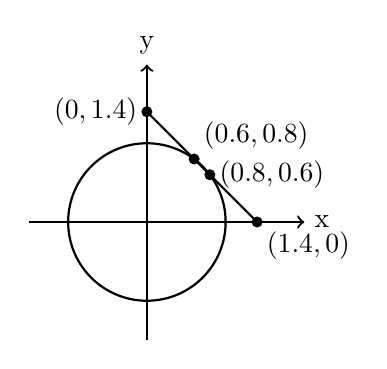
\begin{tikzpicture}
\draw [thick] (0,0) circle (1cm);
\draw [thick] (0,1.4) coordinate (a_1) -- (1.4,0) coordinate (a_2);
\draw [->,thick] (0,-1.5) -- (0,2) node (yaxis) [above] {y};
\draw [->,thick] (-1.5, 0) -- (2, 0) node (xaxis) [right] {x};
\fill[black] (a_1) circle (2pt) node[left] {$(0, 1.4)$};
\fill[black] (a_2) circle (2pt) node[below right] {$(1.4, 0)$};
\fill[black] (0.6,0.8) circle (2pt) node[above right] {$(0.6, 0.8)$};
\fill[black] (0.8,0.6) circle (2pt) node[right] {$(0.8, 0.6)$};
\end{tikzpicture}
\caption{Intersection of $S_{\text{sub}_1}$ and $S_{\text{sub}_2}$}\label{fig11}
\end{figure}

\item Set $S_2$ can be represented as the intersection of two sets $S_{\text{sub}_1} = \{x \in \mathbb{R}^2 | x_1^2 + x_2^2 \leqslant 1 \}$ (which represents closure of a circle) and $S_{\textbf{sub}_2} = \{x \in \mathbb{R}^2 | x_1 + x_2 = 1.5\}$ which is a line. The two sets are shown in Figure \ref{fig12}. As is shown, the two sets do not intersect which means $S_1 = S_{\text{sub}_1} \cap S_{\text{sub}_2} = \emptyset$. Therefore, $K(S) = I(S) = \partial S = \emptyset$.

\begin{figure}[H]\centering
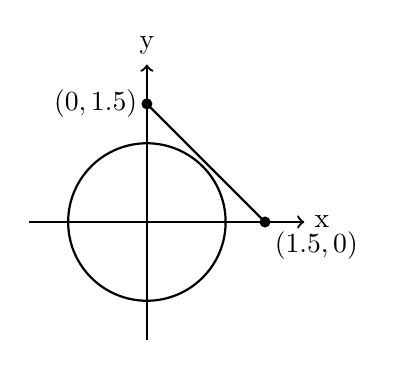
\begin{tikzpicture}
\draw [thick] (0,0) circle (1cm);
\draw [thick] (0,1.5) coordinate (a_1) -- (1.5,0) coordinate (a_2);
\draw [->,thick] (0,-1.5) -- (0,2) node (yaxis) [above] {y};
\draw [->,thick] (-1.5, 0) -- (2, 0) node (xaxis) [right] {x};
\fill[black] (a_1) circle (2pt) node[left] {$(0, 1.5)$};
\fill[black] (a_2) circle (2pt) node[below right] {$(1.5, 0)$};
\end{tikzpicture}
\caption{$S_{\text{sub}_1}$ and $S_{\text{sub}_2}$}\label{fig12}
\end{figure}

We can as well mathematically support our deduction by showing no real solution exists for the following equation.

\begin{equation}
\left\{ \begin{array}{ll} x_1^2 + x_2^2 = 1 \\ x_1 + x_2 = 1.5 \end{array} \right.
\label{eq12}
\end{equation}

Eq. \ref{eq12} translates to $2x_2^2 - 3x_2 + 1.25 = 0$ and yields to $x_2 = 0.75 + 0.25j$ and $x_2 = 0.75 - 0.25j$ which shows the two sets never intersect.

\end{enumerate}
